During the training with PCC loss the model has successfully converged already after 35 epochs, however a clear overfit was encountered (see Figure \ref{fig:er-overfit}a) with the best PCC loss before the overfit being $0.0713$. Overfitting happens due to the lack of data, as for the case of ER there were much fewer samples than for nuclei for example (see Table \ref{table:data}). Even though one could use an early-stopping approach and simply choose an earlier epoch before overfit, the better approach would be to use regularization methods described in section \ref{section:regularization}. In this case data augmentations (flipps and scale crops) were introduced. The new learning curve is shown in Figure \ref{fig:er-overfit}b. Overfit now happens much later (after $120$ epochs) and PCC loss improves to $0.0701$. Introducing a stronger regularization with the use of weight decay in adadelta optimizer and dropout layers with a dropout rate of $0.1$ (see Figure \ref{fig:er-overfit}c) reduces the overfit completely, however at the same time increases the loss to $0.099$.
\begin{figure}[H]
	\begin{center}
		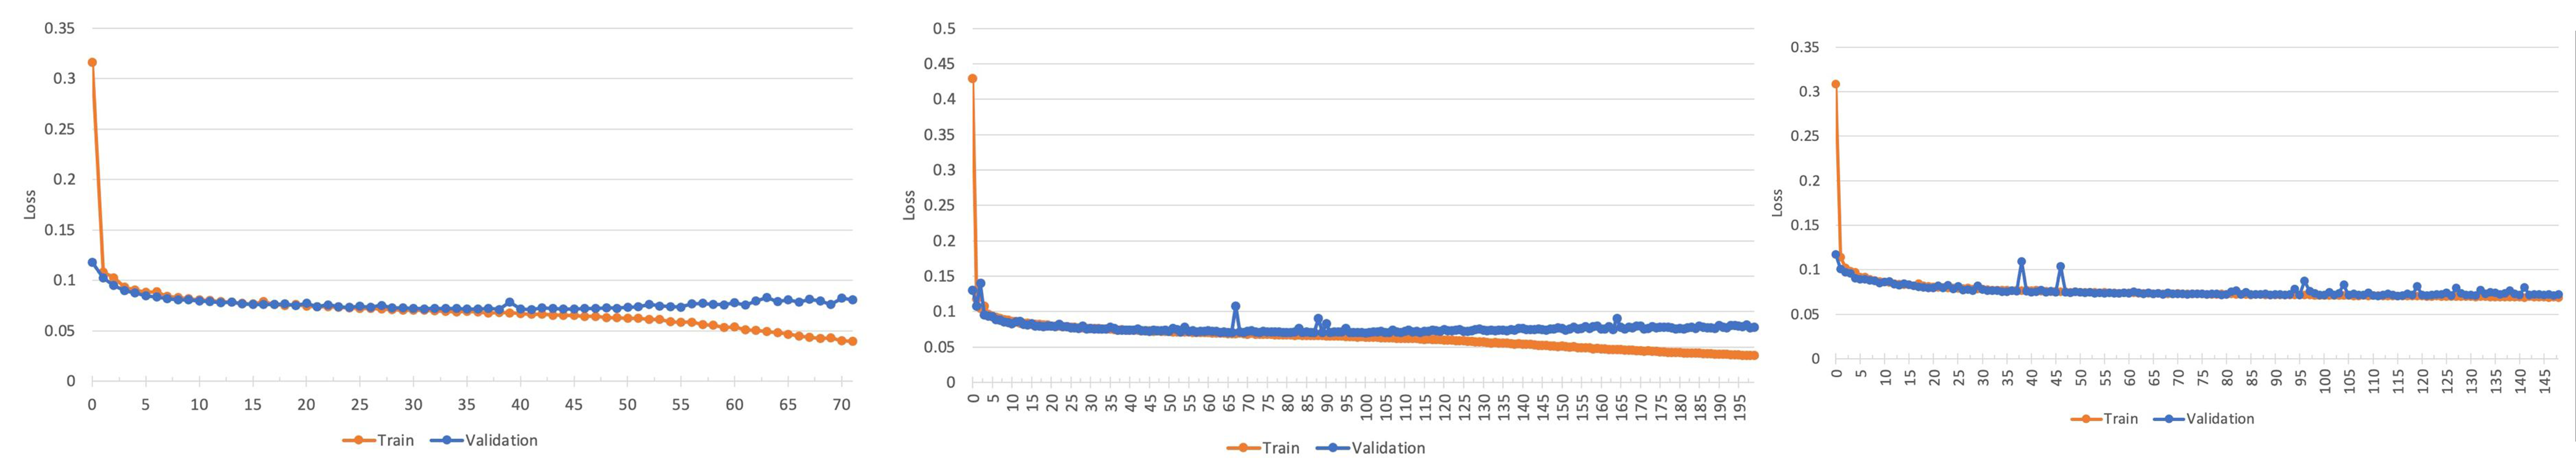
\includegraphics[width=\linewidth]{bilder/ER/segmentation/reg-not-reg.png}
		\caption{Default model (left), slightly regularized model (middle), strongly regularized model (right)}\label{fig:er-overfit}
	\end{center}
\end{figure}

From the fact that the loss has increased too strong with the use of weight decay, it can be concluded that such regularization approach was too strong. In this case it is better to use early-stopping approach with the epoch that has the lowest losd and as a result the model trained with augmentations only was chosen.

%Although the validation loss seems to be higher in comparison to $0.0701$, in this case the growths were not explained by the difference between the validation sets, where the loss was measured on. PCC losses on the same validation set for both were $0.0701$ and $0.0742$.